\begin{frame}[allowframebreaks]{Permutation Invariance}
    \begin{itemize}
        \item \textbf{Positional Encoding:} Supplies sequence order information to models that lack recurrence or convolution, such as Transformers.
        \item Concatenate or add a special positional encoding $p_j$ to each input vector $x_j$.
        \item A function $\mathrm{pos}: \mathbb{N} \rightarrow \mathbb{R}^D$ maps the position $j$ of the vector into a $D$-dimensional vector, i.e., $p_j = \mathrm{pos}(j)$.
    \end{itemize}

    \vspace{1em}

    \begin{figure}
        \centering
        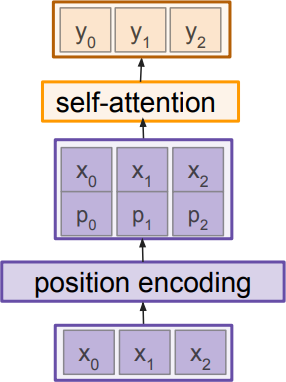
\includegraphics[width=\linewidth,height=0.45\textheight,keepaspectratio]{images/transformers/slide_45_1_img.png}
    \end{figure}

    \framebreak
    \begin{itemize}
        \item The positional encoding is added to the input vectors before computing the attention scores.
        \item This allows the model to incorporate information about the position of each vector in the sequence.
        \item The positional encoding can be learned or fixed, depending on the implementation.
        \item The choice of positional encoding can affect the model's ability to capture long-range dependencies and relationships in the data.
        \item \textbf{Sinusoidal encodings:} Common fixed positional encoding uses sine and cosine functions:
        \begin{align*}
            \mathrm{pos}(j)_{2k} &= \sin\left(\frac{j}{10000^{2k/d}}\right) \\
            \mathrm{pos}(j)_{2k+1} &= \cos\left(\frac{j}{10000^{2k/d}}\right)
        \end{align*}
    \end{itemize}
\end{frame}